\documentclass[letterpaper, 10pt, conference, twoside]{ieeeconf}


\IEEEoverridecommandlockouts
\overrideIEEEmargins
\usepackage{ctex}
\usepackage{booktabs}
\usepackage{graphicx}
\graphicspath{{figures/}}%图片所在的目录

\usepackage{lastpage}%获得总页数
\usepackage{fancyhdr}
\pagestyle{fancy}
%以下命令中L--左侧 R--右侧 C--中间 O--奇数页 E--偶数页
%\fancyhead[LO,RE]{机器学习原理、工程技术与应用}%奇数页左侧,偶数页右侧显示页眉
\fancyhead[CO,RE]{机器学习}%奇数页左侧,偶数页右侧显示页眉
\fancyhead[LO,CE]{代课教师 李乡儒,华南师范大学计算机学院}%奇数页左侧,偶数页中间页脚为空
\fancyhead[RO,LE]{\today}%奇数页右侧,偶数页左侧显示 当前页 of 总页数
\fancyfoot[CO,RE]{机器学习}%奇数页中间,偶数页右侧页脚为空
\fancyfoot[LO,CE]{2021-2022-2学期}%奇数页左侧,偶数页中间页脚为空
\fancyfoot[RO,LE]{\thepage\ of \pageref{LastPage}}%奇数页右侧,偶数页左侧显示 当前页 of 总页数
\renewcommand{\headrulewidth}{0.4pt}%改为0pt即可去掉页眉下面的横线
\renewcommand{\footrulewidth}{0.4pt}%改为0pt即可去掉页脚上面的横线
\setlength{\voffset}{-10mm}
\setlength{\topmargin}{0mm}
\setlength{\headheight}{5mm}
\setlength{\headsep}{5mm}
\setlength{\footskip}{8mm}



\title{\LARGE \bf
机器学习作业模板
}


\author{学号 \quad 姓名\\ \today\\ 机器学习作业}


\begin{document}

\maketitle
%\thispagestyle{empty}
%\pagestyle{empty}



\begin{abstract}
该模板适用于机器学习高级技术及应用课程. 所有地方使用英文状态下的标点符号, 标点符号之后空一个空格.

\vspace{1ex}\noindent\textbf{关键词}: 词1; 词2

\end{abstract}

\begin{eabstract}
	English Abstract
	
\vspace{1ex}\noindent\textbf{Keywords}: word1; word2
\end{eabstract}


\section{一级标题}
\subsection{二级标题}
\subsubsection{三级标题}




\section{图表}

\begin{figure}[htbp]
  \centering
  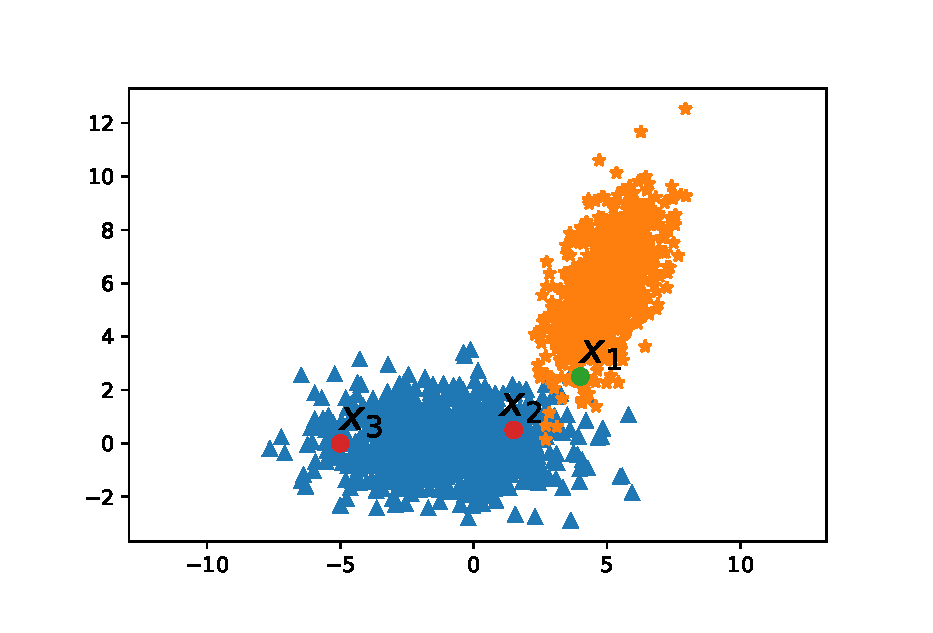
\includegraphics[width = 1\linewidth]{smooth}
  \caption{图片名称及图片内容简介}
  \label{fig:fig1}
\end{figure}


\begin{table}[htbp]
  \centering
 \caption{三线表}
 \label{tab:table2}
 \begin{tabular}{llll}
  \toprule
  表头1 & 表头2 & 表头3& 表头4\\
  \midrule
    模&式&识&别\\
    机&器&学&习\\
    数&据&挖&掘\\
    人&工&智&能\\
  \bottomrule
 \end{tabular}
\end{table}




\section{列点}

\begin{itemize}
\item The word ÒdataÓ is plural, not singular.
\item The subscript for the permeability of vacuum ?0, and other common scientific constants, is zero with subscript formatting, not a lowercase letter ÒoÓ.
\end{itemize}

\begin{enumerate}
\item The word ÒdataÓ is plural, not singular.
\item The subscript for the permeability of vacuum ?0, and other common scientific constants, is zero with subscript formatting, not a lowercase letter ÒoÓ.
\end{enumerate}


\section{脚注}
机器学习\footnote{脚注内容}

\section{列点}

\begin{itemize}
\item The word ÒdataÓ is plural, not singular.
\item The subscript for the permeability of vacuum ?0, and other common scientific constants, is zero with subscript formatting, not a lowercase letter ÒoÓ.
\end{itemize}

\begin{enumerate}
\item The word ÒdataÓ is plural, not singular.
\item The subscript for the permeability of vacuum ?0, and other common scientific constants, is zero with subscript formatting, not a lowercase letter ÒoÓ.
\end{enumerate}


\section{列点}

\begin{itemize}
\item The word ÒdataÓ is plural, not singular.
\item The subscript for the permeability of vacuum ?0, and other common scientific constants, is zero with subscript formatting, not a lowercase letter ÒoÓ.
\end{itemize}

\begin{enumerate}
\item The word ÒdataÓ is plural, not singular.
\item The subscript for the permeability of vacuum ?0, and other common scientific constants, is zero with subscript formatting, not a lowercase letter ÒoÓ.
\end{enumerate}


\section{列点}

\begin{itemize}
\item The word ÒdataÓ is plural, not singular.
\item The subscript for the permeability of vacuum ?0, and other common scientific constants, is zero with subscript formatting, not a lowercase letter ÒoÓ.
\end{itemize}

\begin{enumerate}
\item The word ÒdataÓ is plural, not singular.
\item The subscript for the permeability of vacuum ?0, and other common scientific constants, is zero with subscript formatting, not a lowercase letter ÒoÓ.
\end{enumerate}


\section{列点}

\begin{itemize}
\item The word ÒdataÓ is plural, not singular.
\item The subscript for the permeability of vacuum ?0, and other common scientific constants, is zero with subscript formatting, not a lowercase letter ÒoÓ.
\end{itemize}

\begin{enumerate}
\item The word ÒdataÓ is plural, not singular.
\item The subscript for the permeability of vacuum ?0, and other common scientific constants, is zero with subscript formatting, not a lowercase letter ÒoÓ.
\end{enumerate}

\section{列点}

\begin{itemize}
\item The word ÒdataÓ is plural, not singular.
\item The subscript for the permeability of vacuum ?0, and other common scientific constants, is zero with subscript formatting, not a lowercase letter ÒoÓ.
\end{itemize}

\begin{enumerate}
\item The word ÒdataÓ is plural, not singular.
\item The subscript for the permeability of vacuum ?0, and other common scientific constants, is zero with subscript formatting, not a lowercase letter ÒoÓ.
\end{enumerate}


\section{列点}

\begin{itemize}
\item The word ÒdataÓ is plural, not singular.
\item The subscript for the permeability of vacuum ?0, and other common scientific constants, is zero with subscript formatting, not a lowercase letter ÒoÓ.
\end{itemize}

\begin{enumerate}
\item The word ÒdataÓ is plural, not singular.
\item The subscript for the permeability of vacuum ?0, and other common scientific constants, is zero with subscript formatting, not a lowercase letter ÒoÓ.
\end{enumerate}

\section{列点}

\begin{itemize}
\item The word ÒdataÓ is plural, not singular.
\item The subscript for the permeability of vacuum ?0, and other common scientific constants, is zero with subscript formatting, not a lowercase letter ÒoÓ.
\end{itemize}

\begin{enumerate}
\item The word ÒdataÓ is plural, not singular.
\item The subscript for the permeability of vacuum ?0, and other common scientific constants, is zero with subscript formatting, not a lowercase letter ÒoÓ.
\end{enumerate}

\section{列点}

\begin{itemize}
\item The word ÒdataÓ is plural, not singular.
\item The subscript for the permeability of vacuum ?0, and other common scientific constants, is zero with subscript formatting, not a lowercase letter ÒoÓ.
\end{itemize}

\begin{enumerate}
\item The word ÒdataÓ is plural, not singular.
\item The subscript for the permeability of vacuum ?0, and other common scientific constants, is zero with subscript formatting, not a lowercase letter ÒoÓ.
\end{enumerate}

\section{列点}

\begin{itemize}
\item The word ÒdataÓ is plural, not singular.
\item The subscript for the permeability of vacuum ?0, and other common scientific constants, is zero with subscript formatting, not a lowercase letter ÒoÓ.
\end{itemize}

\begin{enumerate}
\item The word ÒdataÓ is plural, not singular.
\item The subscript for the permeability of vacuum ?0, and other common scientific constants, is zero with subscript formatting, not a lowercase letter ÒoÓ.
\end{enumerate}

\section{列点}

\begin{itemize}
\item The word ÒdataÓ is plural, not singular.
\item The subscript for the permeability of vacuum ?0, and other common scientific constants, is zero with subscript formatting, not a lowercase letter ÒoÓ.
\end{itemize}

\begin{enumerate}
\item The word ÒdataÓ is plural, not singular.
\item The subscript for the permeability of vacuum ?0, and other common scientific constants, is zero with subscript formatting, not a lowercase letter ÒoÓ.
\end{enumerate}

\section{列点}

\begin{itemize}
\item The word ÒdataÓ is plural, not singular.
\item The subscript for the permeability of vacuum ?0, and other common scientific constants, is zero with subscript formatting, not a lowercase letter ÒoÓ.
\end{itemize}

\begin{enumerate}
\item The word ÒdataÓ is plural, not singular.
\item The subscript for the permeability of vacuum ?0, and other common scientific constants, is zero with subscript formatting, not a lowercase letter ÒoÓ.
\end{enumerate}

\section{列点}

\begin{itemize}
\item The word ÒdataÓ is plural, not singular.
\item The subscript for the permeability of vacuum ?0, and other common scientific constants, is zero with subscript formatting, not a lowercase letter ÒoÓ.
\end{itemize}

\begin{enumerate}
\item The word ÒdataÓ is plural, not singular.
\item The subscript for the permeability of vacuum ?0, and other common scientific constants, is zero with subscript formatting, not a lowercase letter ÒoÓ.
\end{enumerate}


\begin{thebibliography}{99}

\bibitem{c1} G. O. Young, ÒSynthetic structure of industrial plastics (Book style with paper title and editor),Ó 	in Plastics, 2nd ed. vol. 3, J. Peters, Ed.  New York: McGraw-Hill, 1964, pp. 15Ð64.
\bibitem{c2} W.-K. Chen, Linear Networks and Systems (Book style).	Belmont, CA: Wadsworth, 1993, pp. 123Ð135.

\end{thebibliography}
\end{document}
